% template file include
% A4 lap méret, 12 pontos betűméret
\documentclass[12pt,a4paper]{article}

% szükséges csomagok
\usepackage[utf8]{inputenc}
\usepackage[T1]{fontenc}
\usepackage[magyar]{babel}
\usepackage{float}
\usepackage{graphicx}
\usepackage{pdfpages}
\usepackage{caption}
\usepackage[colorlinks=false, pdfborder={0 0 0}, linkcolor=black, unicode]{hyperref}
\usepackage{mathtools}
\usepackage{relsize}
\usepackage{amsmath}
\usepackage{amsfonts}
\usepackage{amssymb}
\usepackage{listings}
\usepackage{csquotes}
\usepackage{enumitem}
\usepackage{url}
\usepackage[nottoc,numbib]{tocbibind}
\usepackage{titlesec}
\usepackage{titletoc}
\usepackage{textcomp}
\usepackage{gensymb}

% lista elemek közti hely, és vonal mint lista elem előtti jel beállítása
\setlist{nosep, label={--}}

% tartalomjegyzék formázása
\dottedcontents{section}[1.5em]{}{1.5em}{1pc}
\dottedcontents{subsection}[3em]{}{2em}{1pc}
\dottedcontents{subsubsection}[5em]{}{3em}{1pc}

% fejezet cím formázás: 14 pontos betűméret, nagybetűs
\titleformat{\section}{\normalfont\fontsize{14}{14}\mdseries\MakeUppercase}{\thesection}{1em}{}
\titleformat{\subsection}{\normalfont\fontsize{12}{12}\bfseries}{\thesubsection}{1em}{}
\titleformat{\subsubsection}{\normalfont\fontsize{12}{12}\bfseries}{\thesubsubsection}{1em}{}

% fejezet cím térközök
\titlespacing*{\section}{0em}{0em}{1em}
\titlespacing*{\subsection}{0em}{1em}{1em}
\titlespacing*{\subsubsection}{0em}{1em}{1em}


% margó
\usepackage[right=2.50cm, 
            left=3.50cm, 
            top=2.50cm, 
            bottom=4.00cm
            ]{geometry}

% sorköz
\linespread{1.15}

% times new roman betűtípus
\usepackage{times}

% ábra és táblázat számozás beállítása fejezetenként
\setcounter{figure}{0}
\renewcommand{\thefigure}{\arabic{section}.\arabic{figure}}
\setcounter{table}{0}
\renewcommand{\thetable}{\arabic{section}.\arabic{table}}
\numberwithin{equation}{section}
\numberwithin{figure}{section}

% ábra, táblázat cím formázás
\captionsetup[figure]{labelfont={it, small},textfont={it, small},labelsep=colon}
\captionsetup[table]{labelfont={it, small},textfont={it, small},labelsep=colon}

% hivatkozások formátuma és bib fájl importálása
\usepackage[backend=biber,style=ieee,doi=true,isbn=true,url=false,eprint=false]{biblatex}
\addbibresource{references.bib}

% bekezdés behúzása
\setlength{\parindent}{5 mm}

% bekezdés térköz
\setlength{\parskip}{8pt}

% ábra és táblajegyzék formázása
\makeatletter
\renewcommand\listoffigures{
    \section{\listfigurename}
      \@mkboth{\MakeUppercase\listfigurename}%
              {\MakeUppercase\listfigurename}%
    \@starttoc{lof}%
    }

\renewcommand\listoftables{
    \section{\listtablename}
      \@mkboth{\MakeUppercase\listtablename}%
              {\MakeUppercase\listtablename}%
    \@starttoc{lot}%
    }
\makeatother





\begin{document}


\pagenumbering{gobble}

% ELŐLAPOK: borító, feladatlap, nyilatkozat, konzultációs napló

\includepdf[pages=-]{includes/borito.pdf}

\includepdf[pages=-]{includes/feladatlap.pdf}

\includepdf[pages=-]{includes/nyilatkozat.pdf}
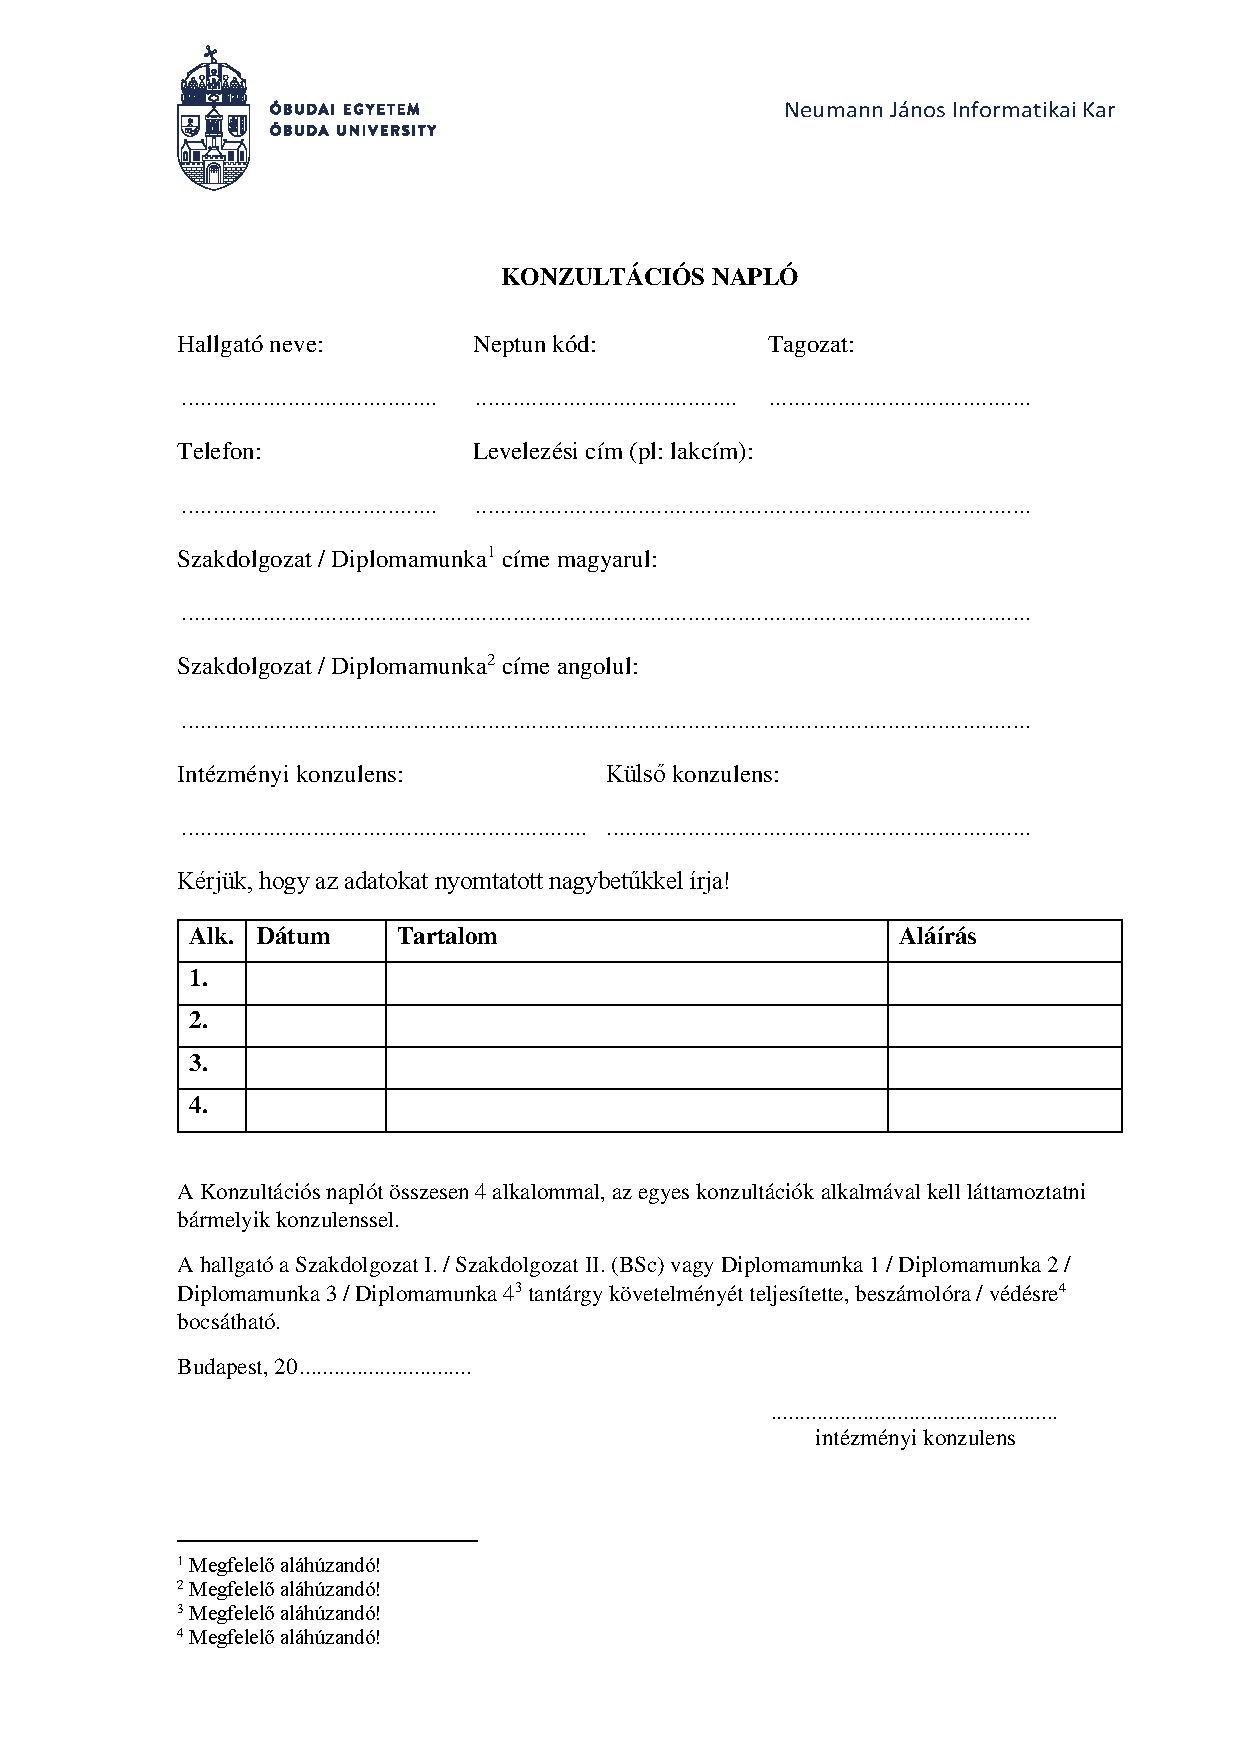
\includepdf[pages=-]{includes/konzultacios_naplo.pdf}


\newpage
\tableofcontents
\newpage

% csak a tartalomjegyzék után kezdődik a számozás
\pagenumbering{arabic}


% -----------------------------------------------------

% ITT KELL HOZZÁADNI A FEJEZETEKET, CÍM NAGYBETŰVEL:

\clearpage
\section{BEVEZETÉS}
Diplomamunka template.

\subsection{Példa alfejezet}
Lorem ipsum dolor sit amet, consectetur adipiscing elit, sed do eiusmod tempor incididunt ut labore et dolore magna aliqua. Ut enim ad minim veniam, quis nostrud exercitation ullamco laboris nisi ut aliquip ex ea commodo consequat. Duis aute irure dolor in reprehenderit in voluptate velit esse cillum dolore eu fugiat nulla pariatur. Excepteur sint occaecat cupidatat non proident, sunt in culpa qui officia deserunt mollit anim id est laborum.

Lorem ipsum dolor sit amet, consectetur adipiscing elit, sed do eiusmod tempor incididunt ut labore et dolore magna aliqua. Ut enim ad minim veniam, quis nostrud exercitation ullamco laboris nisi ut aliquip ex ea commodo consequat. Duis aute irure dolor in reprehenderit in voluptate velit esse cillum dolore eu fugiat nulla pariatur. Excepteur sint occaecat cupidatat non proident, sunt in culpa qui officia deserunt mollit anim id est laborum.


\subsubsection{Példa al-alfejezet}
Lorem ipsum dolor sit amet, consectetur adipiscing elit, sed do eiusmod tempor incididunt ut labore et dolore magna aliqua. Ut enim ad minim veniam, quis nostrud exercitation ullamco laboris nisi ut aliquip ex ea commodo consequat. Duis aute irure dolor in reprehenderit in voluptate velit esse cillum dolore eu fugiat nulla pariatur. Excepteur sint occaecat cupidatat non proident, sunt in culpa qui officia deserunt mollit anim id est laborum.

\clearpage
\section{PÉLDA FEJEZET}
\subsection{Ábrák}
	
Ez itt a \ref{fig:ur5} ábra.
\begin{figure}[H]
	\centering
	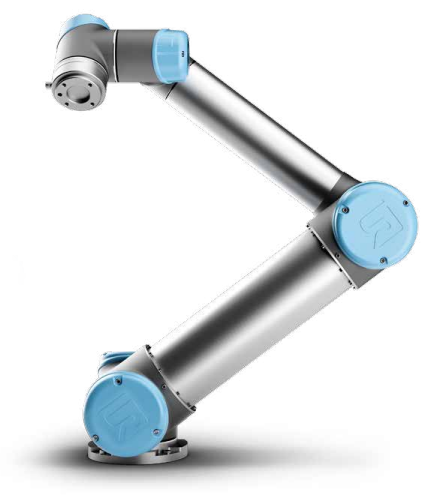
\includegraphics[width=0.5\linewidth]{img/ur5robot.png}
	\caption{UR5 kollaboratív robot}
	\label{fig:ur5}
\end{figure}


\subsection{Hivatkozások}

Ez itt egy folyóirat cikk \cite{journal-example}.

Ez itt egy konferencia cikk \cite{conference-example}.

Ez itt egy könyv \cite{book-example}.

Ez itt egy online forrás \cite{online-example}.

Ez itt egy disszertáció \cite{thesis-example}.

	
\subsection{Táblázatok}
Példaként itt látható egy táblázat \ref{tab:ur5}.

\begin{table}[H]
	\centering
	\begin{tabular}{|c|c|}
	    \hline
		Tulajdonság                      & Érték    \\ \hline
		kinyúlás {[}mm{]}                & 850      \\ \hline
		Szabadságfok                     & 6        \\ \hline
		Teherbírás {[}kg{]}               & 5        \\ \hline
		Súly {[}kg{]}                    & 18,4     \\ \hline
		Ismétlési pontosság {[}mm{]}     & $\pm0,1$    \\ \hline
		Teljesítményfelvétel {[}W{]}     & 90-325   \\ \hline
		Csuklók mozgástartománya {[}$^{\circ}${]} & $\pm360$    \\ \hline
		Max. csuklósebesség {[}$^{\circ}/sec${]}  & $\pm180$    \\ \hline
		Max. Tool sebesség {[}m/s{]}     & 1        \\ \hline
		Programozási nyelv               & URscript \\ \hline
	\end{tabular}
	\caption{Az UR5 robot főbb paraméterei}
	\label{tab:ur5}
\end{table}

Egy másik a \ref{tab:joint-limits} táblázat.

\begin{table}[H]
    \centering
    \begin{tabular}{|c|c|c|c|c|}
        \hline
    	Robotcsukló & \begin{tabular}[c]{@{}c@{}}min. poz.\\ {[}rad{]}\end{tabular} & \begin{tabular}[c]{@{}c@{}}max. poz.\\ {[}rad{]}\end{tabular} & \begin{tabular}[c]{@{}c@{}}max. sebesség\\ {[}rad/s{]}\end{tabular} & \begin{tabular}[c]{@{}c@{}}max. gyorsulás\\ \hline {[}rad/s\textasciicircum{}2{]}\end{tabular} \\ \hline
    	1 & -0.802 & 1.39 & 3.1 & 9 \\ \hline
    	2 & -2.25 & -0.873 & 3.1 & 9 \\ \hline
    	3 & 1.25 & 2.7 & 3.1 & 9 \\ \hline
    	4 & -3.49 & -1.41 & 3.1 & 9 \\ \hline
    	5 & -2.62 & -0.62 & 3.1 & 9 \\ \hline
    	6 & -3.14 & 2.09 & 3.1 & 9 \\ \hline
    \end{tabular}
    \caption{Másik példa táblázat}
    \label{tab:joint-limits}
\end{table}

	
\subsection{Képlet}

Ez itt a \ref{eq:keplet1} képlet:
\begin{align}
    \cos{\alpha-\beta} = \cos{\alpha}\cdot\sin{\beta}-\cos{\beta}\cdot\sin{\alpha}
    \label{eq:keplet1}
\end{align}	

	
\subsection{Felsorolás}

Ez egy felsorolás:
\begin{itemize}
	\item A felsorolás első eleme
	\item A felsorolás második eleme
	\item A felsorolás harmadik eleme
\end{itemize}










% ------------------------------------------------------

% JEGYZÉKEK, INNEN KI LEHET KOMMENTEZNI AMELYIK ESETLEG NEM KELL (de ha van ábra/táblázat akkor kötelező, irodalomjegyzék kötelező, rövidítések opcionális)

\clearpage
\section{IRODALOMJEGYZÉK}
\printbibliography[heading=none]

\clearpage
\renewcommand{\listfigurename}{ÁBRAJEGYZÉK}
\listoffigures

\clearpage
\renewcommand{\listtablename}{TÁBLAJEGYZÉK}
\listoftables

\clearpage
\section{RÖVIDÍTÉSEK}
\newcommand{\acronym}[2]{
    \item [\textbf{#1}] #2
}

\begin{itemize}[labelwidth=3cm,align=left,itemindent=3cm,itemsep=4pt]

% IDE LEHET HOZZÁADNI A RÖVIDÍTÉSEKET:

    \acronym{UR}{Universal Robots}
    \acronym{ROS}{Robot Operating System}
    \acronym{NASA}{National Aeronautics and Space Administration}

\end{itemize}





\end{document}
